\documentclass[12pt,letterpaper]{article}
\usepackage{natbib}

%Packages
\usepackage{pdflscape}
\usepackage{fixltx2e}
\usepackage{textcomp}
\usepackage{fullpage}
\usepackage{float}
\usepackage{latexsym}
\usepackage{url}
\usepackage{epsfig}
\usepackage{graphicx}
\usepackage{amssymb}
\usepackage{amsmath}
\usepackage{mathtools}
\usepackage{bm}
\usepackage{array}
\usepackage[version=3]{mhchem}
\usepackage{ifthen}
\usepackage{caption}
\usepackage{hyperref}
\usepackage{amsthm}
\usepackage{amstext}
\usepackage{enumerate}
\usepackage[osf]{mathpazo}
\usepackage{dcolumn}
\usepackage{lineno}
\usepackage{dcolumn}
\newcolumntype{d}[1]{D{.}{.}{#1}}

\pagenumbering{arabic}


%Pagination style and stuff
\linespread{2}
\raggedright
\setlength{\parindent}{0.5in}
\setcounter{secnumdepth}{0} 
\renewcommand{\section}[1]{%
\bigskip
\begin{center}
\begin{Large}
\normalfont\scshape #1
\medskip
\end{Large}
\end{center}}
\renewcommand{\subsection}[1]{%
\bigskip
\begin{center}
\begin{large}
\normalfont\itshape #1
\end{large}
\end{center}}
\renewcommand{\subsubsection}[1]{%
\vspace{2ex}
\noindent
\textit{#1.}---}
\renewcommand{\tableofcontents}{}
%\bibpunct{(}{)}{;}{a}{}{,}

%---------------------------------------------
%
%       START
%
%---------------------------------------------

\begin{document}

%Running head
\begin{flushright}
Version dated: \today
\end{flushright}
\bigskip
\noindent RH: Branch swapping algorithm

\bigskip
\medskip
\begin{center}

\noindent{\Large \bf Tree rearrangements rearranged} %TG: I'm bad at puns.
\bigskip

\noindent {\normalsize \sc Thomas Guillerme$^1$$^*$, and Martin D. Brazeau$^1$}\\ %TG: Author order can be swapped of course! There's only a finite combination of 2 elements anyway!
\noindent {\small \it 
$^1$Imperial College London, Silwood Park Campus, Department of Life Sciences, Buckhurst Road, Ascot SL5 7PY, United Kingdom.\\}
\end{center}
\medskip
\noindent{*\bf Corresponding author.} \textit{t.guillerme@imperial.ac.uk}\\  %TG: Same as above
\vspace{1in}

%Line numbering
\modulolinenumbers[1]
\linenumbers

%---------------------------------------------
%
%       ABSTRACT
%
%---------------------------------------------

\newpage
\begin{abstract}
blablabla
\end{abstract}

\noindent (Keywords: )\\

\vspace{1.5in}

\newpage 


%---------------------------------------------
% LaTeX tips for modifying/editing the document:
%---------------------------------------------
% - You can comment using the percentage sign. I suggest you use the % sign alone for commenting out sections of the text:
%       e.g. "This is a really long sentence %because this sentence is very long." Here the % is used for ignoring the end of the sentence (but for some reason you want to keep track of it).%
%       For comments as in verbose comments, I suggest you use "%MB:":
%       e.g. "This is a really long sentence %because this sentence is very long. %MB: yeah, no shit!" 
% - For optimal version control, write only one sentence per line (for more precise track changes)
% - To build the pdf, use command+B in Sublime.
% - Because of the bibliography, the pdf needs to be build in the same folder that contains "References.bib" and "sysbio.bst"
% - For citing papers, you must put their bibtex reference in the "References.bib" file and then you can use the following sysbio tags:
%        \cite{bibtexBob2000} for citing within a sentence: "Bob (2000)"
%        \citep{bibtexBob2000} for citing within brackets: "(Bob, 2000)"
%        \citep[Before:][-After]{bibtexBob2000} for citing within brackets with additional text: "(Before: Bob, 2000 -After)"
%        \citealt{bibtexBob2000} for citing without brackets: "Bob, 2000"
%        You can put more cites in each \cite tag by separating them with commas.
% - For equation, find every details here: https://en.wikibooks.org/wiki/LaTeX/Mathematics
% - For titles and stuff, the hierarchy goes \section{}, \subsection{}, \subsubsection{} and so forth...
% - For bullet points or enumerations you can use:
%       \begin{itemize}
%           \item my first bullet point/enumeration
%       \end{itemize}
%       With replacing "itemize" by "enumerate" for enumeration.




%---------------------------------------------
%
%       INTRODUCTION
%
%---------------------------------------------
\section{Introduction}

% Tree rearrangement is paramount
Phylogenetic studies are confronted with the combinatoric problem of intractably large numbers of tree solutions arising from increasing numbers of terminals \citep{Felsenstein:1978vh}.
%TG: maybe we could replace "terminals" by "taxa"? Seems a bit less mathsy.
To address this problem, heuristic solutions involving tree rearrangements permit exploration of restricted parts of ``tree space'' close to target solutions.
This greatly accelerates phylogenetic analysis by ignoring topologies that are unlikely to be optimal.
In addition to their use in the phylogenetic tree search process itself, tree rearrangement strategies are employed in some post-search tasks such as tree comparisons \citep[e.g.][]{allen2001subtree,kuhner2015treComparison}, node support estimation \citep[e.g.][]{goloboff2014bias} or methods for detecting horizontal genes transfer \citep[e.g.][]{mcfadden1995something,bordewich2005computational}.

Recently, \citet{goloboff2014bias} examined biases in tree searches arising from heuristic methods, noting in particular how these biases can influence support statistics including bootstrap values and posterior probabilities arising from %Markov chain results.
Bayesian inference. %TG: the posterior probabilities are calculated from Bayes theorem, the MCMC is just a way to get there. I think.
They note that the biases are amplified if branch-swapping procedures do not take care to avoid redundant swaps (Fig.\ref{Figure_1}).
Additionally, the speed and efficiency of branch-swapping strategies is of critical importance.
Considerable time should be saved by not visiting topologies that have already been analysed.
However, the question of how redundant swaps are avoided may not be immediately obvious from the explanations given in most texts \citep{swofford2003phylogeny,felsenstein2004inferring,wiley2011phylogenetics}.
The explanations given for branch-swapping algorithms (reviewed below) given in most popular texts and reviews will almost certainly result in redundant topologies within even the same round of branch swapping.

\begin{figure}[!htbp]
\centering
   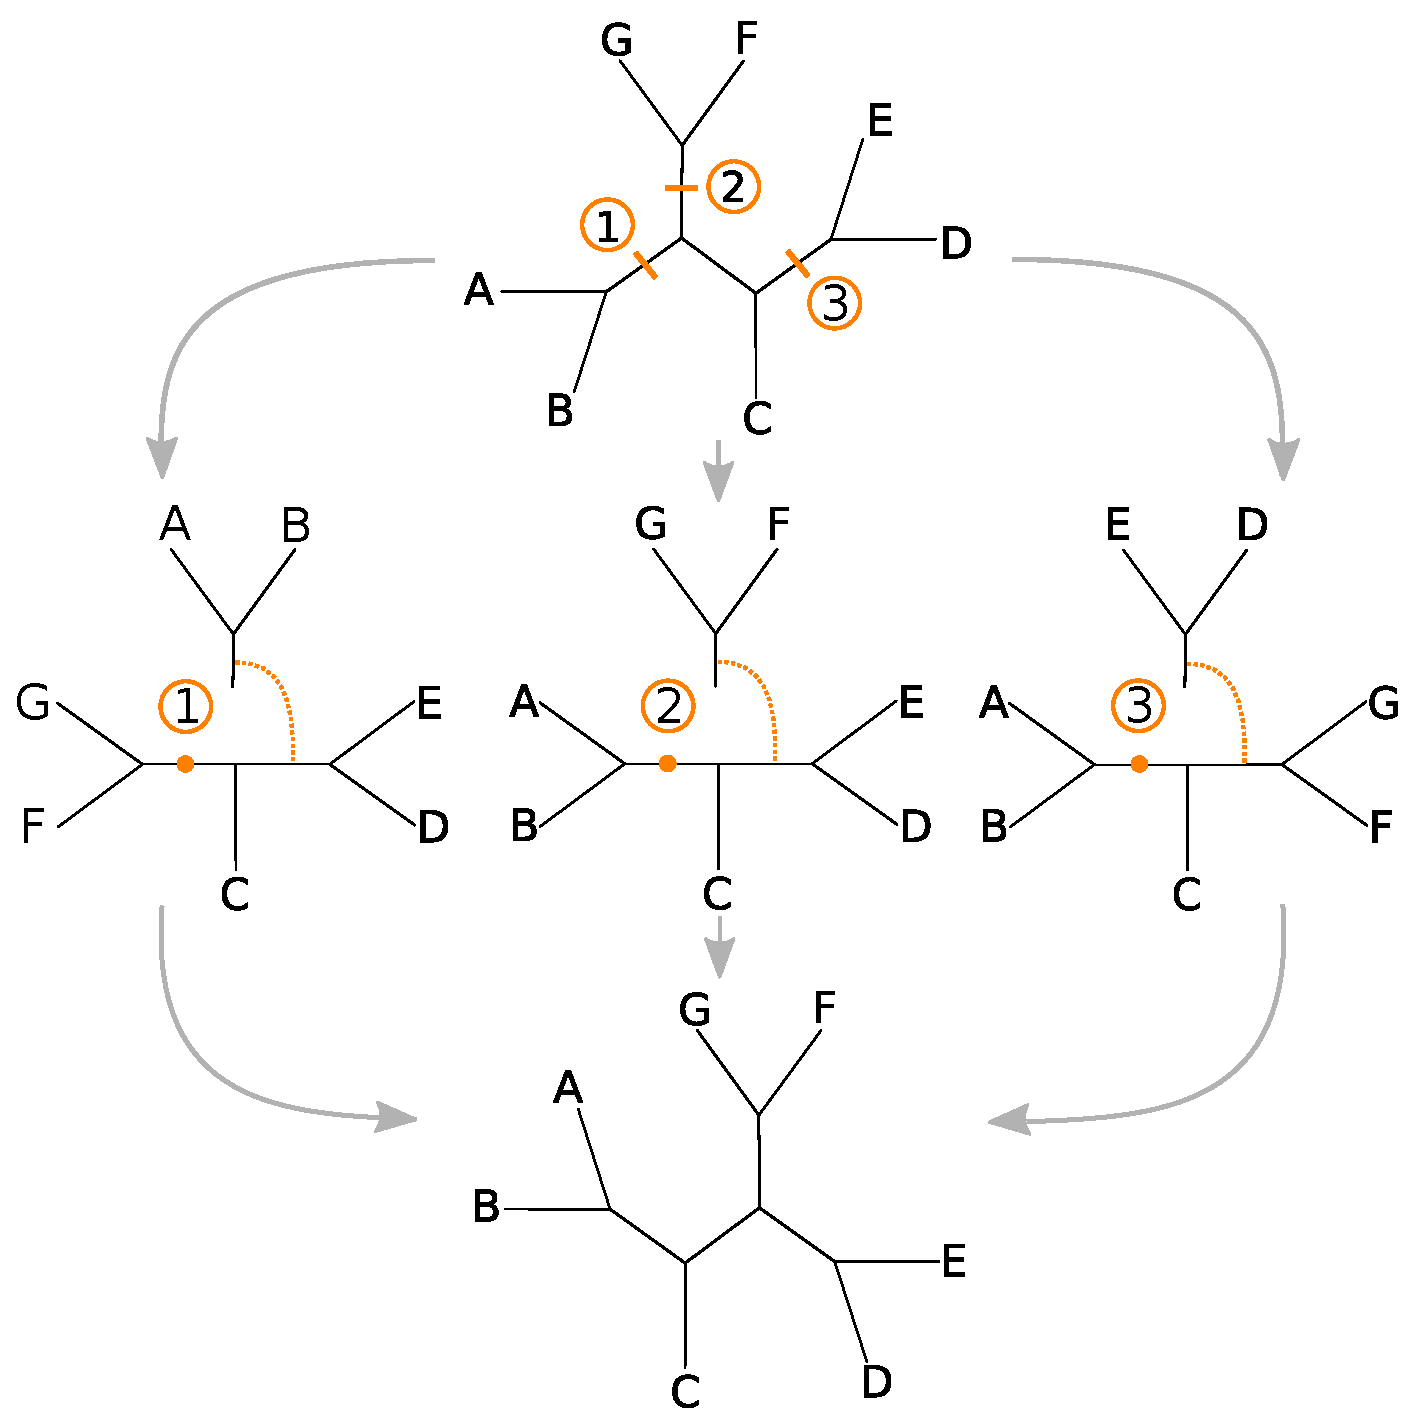
\includegraphics[width=0.9\textwidth]{Figure/Figure_RedundantSwaps.pdf}
\caption{Example of redundant swaps. Three independent pruning (clades ``(A,B)'', ``(G,F)'' and ``(E,D)'') and regrafting (orange doted line) leads to the exact same topology. The orange dots represents the clades original position.}
\label{Figure_1}
\end{figure}

How then are redundant swaps avoided? %TG: Maybe something like: "This leads to the lack of clear explanation on how to avoid redundant swaps."
In this review, we provide more precise explanations of subtree pruning and regrafting (SPR) and tree-bisection and reconnection (TBR) rearrangement strategies that result only in unique tree topologies within a single round. 
These explanations account for the order in which branches are broken as well as the pattern in which subtrees are reconnected to the target tree.
We do not claim credit for these methods -- they, or something equivalent to them must already be implemented in existing phylogenetic software.
Furthermore, they are implicit in some mathematical accounts of branch-swapping processes in which the number of unique 1-move rearrangements are counted \citep{allen2001subtree}.% TG: is that what you meant with [EXAMPLES]?
However, we provide an explicit, verbose account that would be useful in assisting any investigators who need to program such routines for the first time. 
We acknowledge that few may need to do this, however we follow \citet{goloboff1993character} in that knowledge of underlying routines helps to foster refinements and improvements of existing strategies that have a large user base. %TG: not sure about the "few needs to know" part. It's kind of auto-diminishing the impact of the paper. Maybe we can go with something like:
%We believe that these explanation will help researchers using phylogenetic to better understand the underlying search routines \citep{goloboff1993character} and can foster refinement and improvement for implementing branch swapping strategies for tree inference or post-tree analysis \citep[e.g.][]{bordewich2005computational,goloboff2014bias,kuhner2015treComparison}.


%MB I'm really not sure this section is needed, but I'll leave it for now. It might be possible to fit it in.
%MB For now, it's mainly a digression from the main point: only unique 1-move swaps from a starting tree
Two main points need to be considered for the reliability of tree arrangement algorithms:
\begin{enumerate}
    \item First, when the tree search only visits some possible solutions this can create problems by having a higher probability of visiting a specific tree topology island since the probability of obtaining any topology by tree rearrangement will not be equal (some topologies might be more visited by chance).
    More concretely, for a tree with $n$ taxa, tree rearrangement algorithms can produce $M$ topologies including $m$ similar ones.
    If the tree search algorithm is set to subsample $m$ topologies only, it can possibly only subsample the $m$ similar topologies thus being ineffective at exploring tree space \citep{allen2001subtree}.
    \item Second, the order in which the possible tree rearrangement topologies are visited is also paramount.
    In fact, to avoid any statistical bias, the visiting order should be strictly random \citep{goloboff2014bias} although, in practice, and for algorithm speed reasons, this is rarely the case (e.g. using post/pre-order traversals [CITE]).
    This as been shown to introduce several biases in theoretical examples \citep{goloboff2014bias} although, to our knowledge, has not been demonstrated empirically.
\end{enumerate}

%MB We therefore need some good algorithms.
%MB Boring! (Not that what follows is terribly exciting) This isn't a paper about needing good algorithms, it's a paper about how to implement some good algorithms correctly (or efficiently?). %TG: agree
Also the way the trees are visited (see point 2 above) modifies the efficiency of these algorithms.
For example, \cite{lakner2008efficiency} found, for Bayesian inference, that SPR (when sampled randomly) was more efficient than TBR (when sampled non-randomly) which was in turn more efficient than SPR (when sampled non-randomly).
%TG: that 


The tree inference literature contains thorough and precise descriptions of both the algorithms \citep[e.g.][]{allen2001subtree,felsenstein2004inferring} and their caveats \citep[i.e speed and reliability - e.g.][]{morrison2007increasing,lakner2008efficiency,goloboff2014bias}.
However, the \textit{implementation} of the algorithms is often overlooked.
Here, we will review two common branch rearrangement algorithms (SPR and TBR) and propose a more practical and intuitive definition of the algorithms that we believe can help their implementation.
It is important to note that the algorithms described here are mathematically equivalent to the ones described in \cite{allen2001subtree} and \cite{felsenstein2004inferring} and we thus do not claim priority or originality on this method that as certainly already be implemented in many softwares and was ``discovered'' empirically by many coders.
%TG: add something about writing code for humans not computers? (i.e. non-cryptic/obfuscating coding practices)

\section{SPR and TBR described in literature}

% \subsection{Tree elements definition}
% \begin{itemize}
%     \item a \textbf{tip} is any leaf of the tree (degree 1 vertices) that is connected to only one node.
%     \item a \textbf{node} is formed by the connection of tips or nodes. In a binary tree, a node has exactly one ancestor (or parent) and two descendants.
%     \item an \textbf{edge} is any single connection between two nodes or a node and a tip.
%     \item the \textbf{root} is the single edge that is only connected to one node (and nothing).
% \end{itemize}
% Any bifurcating (i.e. fully resolved) tree with $n$ tips has $2n-1$ nodes and $2n-2$ edges ($n-2$ internal ones) if rooted and $2n-2$ nodes and $2n-3$ edges ($n-3$ internal ones) if unrooted.

% Definitions: \cite{allen2001subtree,felsenstein2004inferring}

The subtree pruning and regrafting method is commonly described as breaking a tree into to two subtrees and reinserting \textit{one} of these subtrees---the source tree---into all non-redundant positions on the other tree (termed the target tree).
In some explanations the target tree is then reinserted into all available positions on the source subtree (e.g. Swofford and Sullivan, fig. 8.5).
However, if all possible subtrees are clipped and reinserted exactly according to the rules described, then they will always generate redundant trees[FIGURE1].
In many cases, branch breaking and swapping would continue, long after the number of non-redundant topologies has been exhausted, wasting valuable computational time.

TBR differs from SPR in that the source subtree is reinserted before reconnection to the target tree.
Thus TBR and SPR are seen to differ only in that rerooting of the subtree only takes place in TBR.
All possible rerootings of the source subtree are attempted before the next clipping is made.
Because the SPR is a strict subset of TBR moves on any given bifurcating tree, then the problem described here holds as well for TBR.
In either case, it is clear that not all possible branch breakings and reinsertions need to be attempted.


% \begin{figure}[!htbp]
% \centering
%    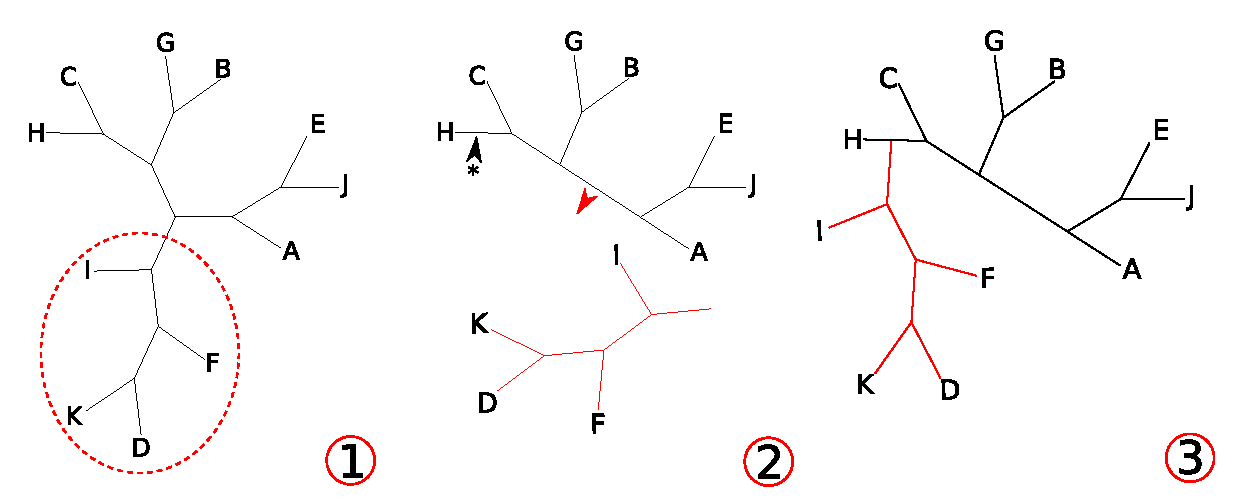
\includegraphics[width=0.9\textwidth]{Figure/SPR.pdf}
% \caption{Suptree Pruning and Regrafting (SPR). Modified from \cite{felsenstein2004inferring}, Figure 4.5. \textbf{1}: a random subtree with $n$ tips is selected; \textbf{2}: the red arrow designates the edge where the subtree was previously branched and the black one the new insertion point. Note that all the edges but the one with the red arrow are potential insertion points. \textbf{3}: the new topology obtained by one SPR rearrangement.}
% \label{Figure_SPR}
% \end{figure}

\section{The Target and Source Tree}
What defines the target and source trees? 
When a subtree is removed from a parent tree and reconnected to various points on the remaining subtree, they implicitly become source and target trees, respectively.
However, with respect to avoiding redundant swaps, source and target are here redefined with respect to the order of clipping. 

% MDB: At this point, it comes clear to me that a glossary or box text might be a useful supplement to define some terms. Secondly, it will be good for us to settle on a few terms and standardise them across the MS.
Although not all clipping and reinsertion points need to be attempted, all possible non-unique moves do need to be tried. 
Clipping (or the enumeration of possible clipping sites) can be made by completing a tree traversal over the initial parent tree.
However, because the parent trees are usually unrooted in practice, an arbitary starting point needs to be selected.
For the purpose of this paper, we elect the node immediately adjacent to the first enumerated tip (usually tip A).
Thus, the trees are implicitly rooted by the traversal procedure.
Clipping may proceed either in postorder or preorder, but in either case, the recursive traversal concludes at the node in which the traversal was initiated.

Because the tree is now implicitly rooted, we can define target and source trees for SPR and TBR with respect to this pattern.
For the purposes of this paper, the target tree is the subtree that contains the starting point of the tree-clipping traversal.
By extension, therefore, the source tree is the clipped subtree that does not contain the starting point.

% MDB: I think this figure caption is likely to go or be changed? 
% \begin{figure}[!htbp]
% \centering
%    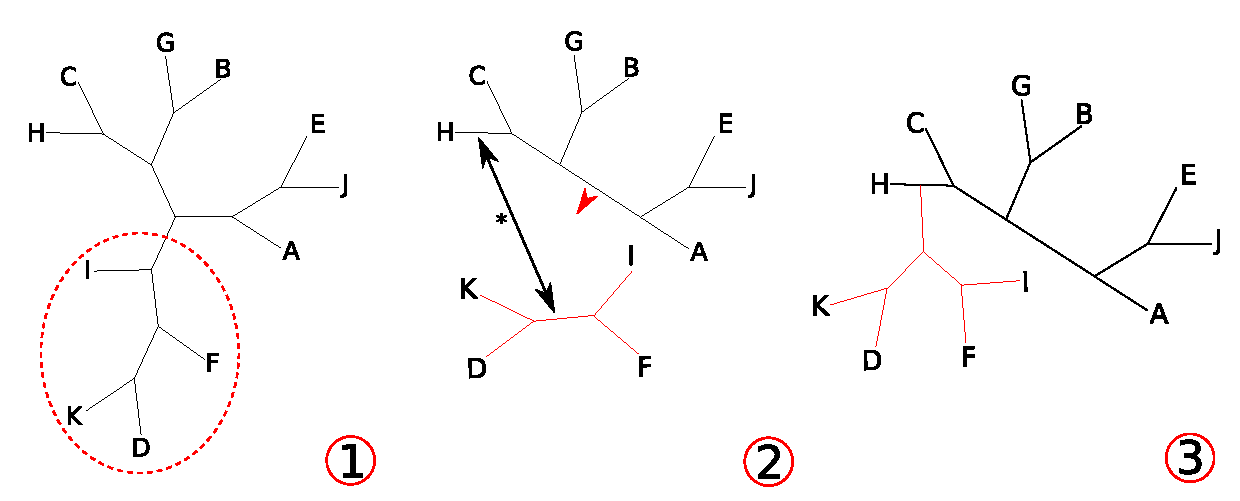
\includegraphics[width=0.9\textwidth]{Figure/TBR.pdf}
% \caption{Tree Bisection and Reconnection (TBR). Modified from \cite{felsenstein2004inferring}, Figure 4.6. \textbf{1}: the trees are split at a random edge and both subtrees are unrooted; \textbf{2}: the red arrow designates the edge where the red tree was previously connected and the black one designates the new rooting point on the red tree and its insertion on the black tree. Note that all the edges on the black tree (but the one with the red arrow) are potential reconnection points. \textbf{3}: the new topology obtained by one TBR rearrangement.}
% \label{Figure_TBR}
% \end{figure}

\section{Patterns Generating Redundant Swaps}
The most obvious case in which a clipping and reconnection procedure results in a redundant topology is the case of reinserting the clipped subtree to its original position.
However, it is trivially easy to avoid these operations.
Figure 1 shows two different clipping and reconnection operations that will result in the same topology. 
What they share in common is that they both result from reinserting the clipped subtree to a branch \textit{neighboring} the original clipping site.

This clips the tree at the smallest subtree that includes both clades. %This is possibly coincidental, but possibly also work thinking about.
Rerooting this clipped subtree on the branch subtending terminal C and reinserting it to the original clipping site generates this same topology.
Conversely, this can be seen as clippling the clade consisting of terminals A and B and reinserting that clade on its neighboring branch (the one subtending C).

We therefore now see three different branch-breaking operations to arrive at the same topology. 
All of them arising from the clipping and moving of a branch to a neighbouring site.
In the next section we show how to employ the order of clipping so that only one of these swaps is made even when the same clipping event occurs.

\section{Avoiding Redundant Swaps}
In the recurring example of redundant swaps from Figures 1 \& 2, we see three possible clipping and reconnection moves that result in the same tree.
However, we only need to commit one of these moves at most once.
All three of these involve clipping a subtree and moving it to a neighbouring branch. 
However, what the first two have in common is that neither clipped tree is the tree containing the starting point of clipping. % I never explicitly defined this, but I think it should be stated as off the node adjacent to A.

In SPR moves, when a branch is clipped, the source tree is reinserted everywhere except the original clipping site \textit{and} any branches immediately adjacent to the original site. 
In turn then, the target tree (containing the traversal starting point) is rejoined to the source tree at all possible points \textit{including} branches neighboring the original clipping site.

For TBR, exactly the same rule follows. 
However, when the source tree is rerooted, it must be reinserted to the original clipping point on the target tree \textit{and} the branches adjacent to it.

\begin{figure}[!htbp]
\centering
   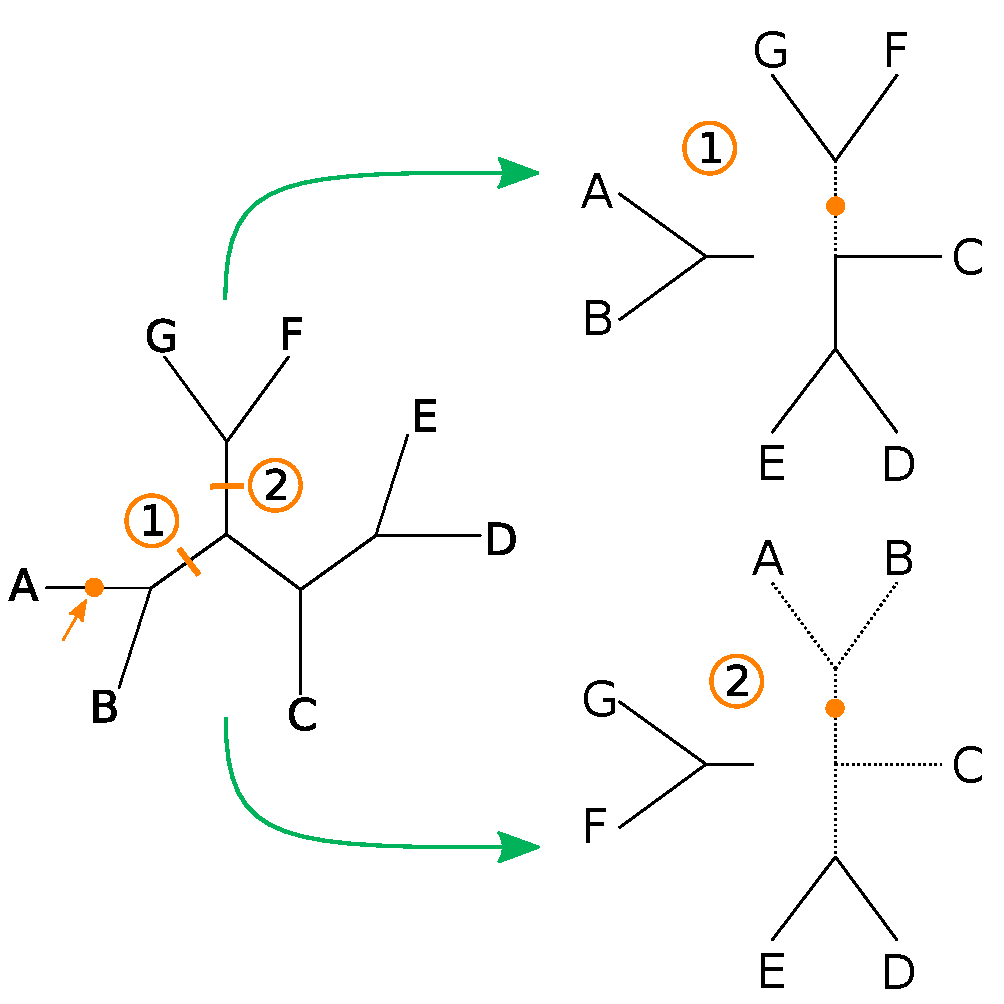
\includegraphics[width=0.7\textwidth]{Figure/Figure_Neighbour.pdf}
\caption{Algorithm illustration for avoiding redundant swaps. If the entry point in the branch swapping traversal is on the tip ``A'' (denoted by the orange arrow), the clade containing the entry point (e.g. ``(A,B)'') can be rebranched everywhere on the target tree (the solid edges) apart from it's previous position (the orange doted line). Any other clades not containing the entry point (e.g. ``(F,G)'') can only be rebranched on edges not adjacent to the original position.}
\label{Figure_SPR}
\end{figure}


% % Dunno if we'll keep the stuff below ##################
% % ######################################################
% \section{Implementation spin}
% These two algorithms can be seen as technically different since they will produce different tree islands, for example, the SPR will, in theory explore fewer topologies than the TBR \citep[see above and][]{morrison2007increasing,lakner2008efficiency}.
% However, once one excludes the visiting of redundant topologies in both algorithms, they can be seen as a generalised way to explore effectively all possible tree topologies.
% First, as described in \cite{allen2001subtree} (but not in \citealt{felsenstein2004inferring}), a simple rule can be applied to avoid redundant topologies in both SPR and TBR algorithm: in both cases the rebranching/reconnection should never occur on the edge of origin (the red arrow in Figs %\ref{Figure_SPR}, \ref{Figure_TBR} and \ref{Figure_TBR_modif}
% ) but neither on the neighbouring ones \citep{allen2001subtree}.
% Second and foremost, an SPR algorithm can be implemented as a TBR one where the rerooting is only done on the edge the closest to the bisection point.% (see Fig \ref{Figure_TBR_modif}).

% % \begin{figure}[!htbp]
% % \centering
% %    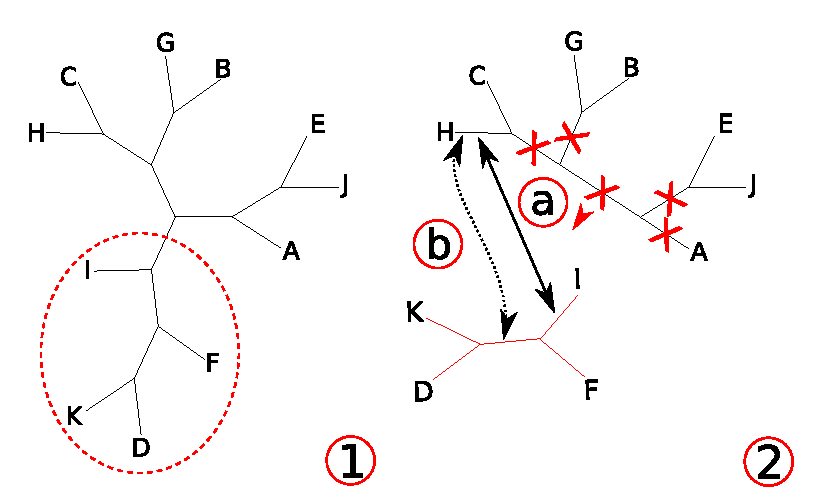
\includegraphics[width=0.9\textwidth]{Figure/TBR_modif.pdf}
% % \caption{Generalised TBR. \textbf{1}: the trees are split at a random edge and both subtrees are unrooted; \textbf{2a}: the red tree is then rooted on the edge closest to the bisection edge and reconnected to an edge on the black tree (i.e. a SPR move); \textbf{2b}: the red tree is rooted on any of its edges and reconnected to an edge on the black tree (i.e. a TBR move). Note that in both cases, the red tree can not be reconnected on the edge of origin (indicated by the red arrow) nor on any of the adjacent edges (marked with a red cross) to avoid any redundant tree rearrangements.}
% % \label{Figure_TBR_modif}
% % \end{figure}



% We believe that such consideration of the SPR algorithm as a constrained TBR highly facilitates both algorithm's implementation.
% In fact, in this case only one algorithm needs to be implemented with one mandatory restricting rules (no reconnection on the bisection edge and it's neighbours) and an optional restriction that can be activate or not to create either TBR or SPR (respectively rerooting on any edge or only on the bisection one).
% This approach is not different than the classic SPR and TBR algorithms described in the literature \citep{allen2001subtree,felsenstein2004inferring} but proposes an easier implementation.

% One of the major concern in phylogenetic inference, during the tree search phase is to evenly (or at worst, randomly) sample the tree space but without spending to much time sampling all possible topologies.
% This allows to identify the different topology islands where the tree search must be focused in order to find the optimal topology.
% One solution to achieve this it to shift between tree rearrangement algorithms during the tree search: first, using an algorithm allowing bold tree rearrangements to explore the overall tree space and then a more conservative one to do a ``fine grain'' search in local optima \citep{lakner2008efficiency}.
% This joint SPR-TBR implementation could easily allow such tree rearrangement shifts by switching between the different restriction rules without implementing different algorithms.
% For example, one could first allow the algorithm to reroot the bissected tree randomly on each of it's edges, creating bolder rearrangements (i.e. exploring the overall tree space) and the constrict the algorithm to only reroot the tree on the edge closest to the bisection edge, creating ``finer grain'' search (i.e. exploring only the SPR island).


%% Glossary %TG: I've added a figure that we can stuck in the supplementary as well
% 
% Tip/Node/Edge
% Original tree: the tree considered for branch swapping operation
% Clipped tree: the sub-tree containing one to n-2 taxa removed from the original tree
% Target tree: the tree that underwent a clipping operation and has now n-1 to n-(n-2) taxa. %TG: we could change that to a more obvious term
% Clipping (to replace: prunning or bissection): removing a sub-tree containing one to n-2 taxa from a tree. The clipping results in obtaining two trees: the clipped tree and the target tree.
% Regrafting/reconnecting: %TG: we should change that to a unique term (same way as clipping, I like reconnecting).
% Swap: one clipping regrafting operation
% Neighbour edge: the edge adjacent to a selcted edge


\section{Acknowledgments}
European Research Council under the European Union’s Seventh Framework Programme (FP/2007–2013)/ERC Grant Agreement number 311092.


\bibliographystyle{sysbio}
\bibliography{References}

\end{document}

